\subsection{Caracterização da transformação martensítica}

\begin{frame}{Resultados}{Caracterização da transformação martensítica no material}
	\begin{columns}
		\begin{column}{7cm}
			\includegraphics<1>[width=7cm]{/home/arthur/texto_tese/img/dilatometria/dil_martensita.pdf}
			\includegraphics<2>[width=7cm]{/home/arthur/texto_tese/img/dilatometria/dil_martensita_close.pdf}
		\end{column}
		\begin{column}<2>{3cm}
				Regra das alavancas:\\
				$$f^{\alpha\text{\textquoteright}} = 1 - f^\gamma = \frac{A}{A + B}$$
		\end{column}
	\end{columns}
\end{frame}

\begin{frame}{Resultados}{Caracterização da transformação martensítica no material}
	\begin{columns}
		\begin{column}{6cm}
			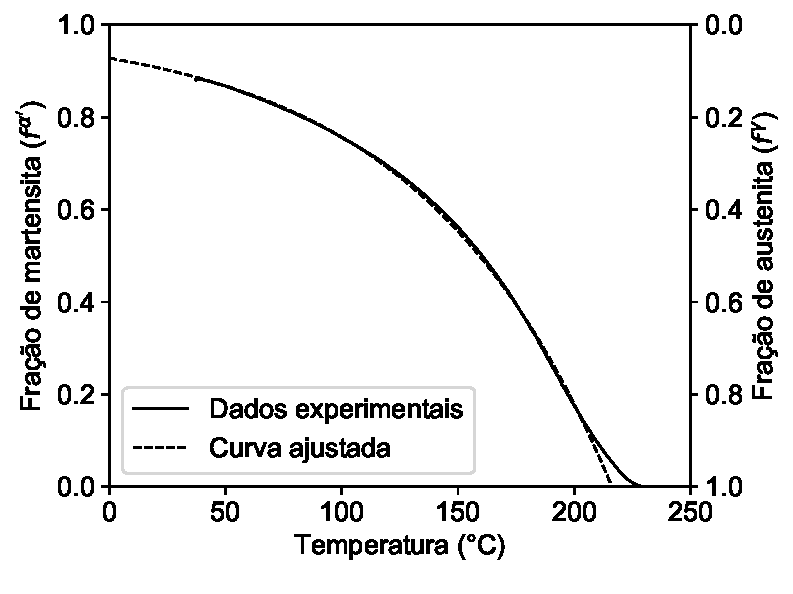
\includegraphics[width=6cm]{/home/arthur/texto_tese/img/dilatometria/frac_martensita.pdf}
		\end{column}
		\begin{column}{4cm}
			\begin{tabular}{c c}
			\hline
			TT [°C] & $f^\gamma$ (\% vol)\\
			\hline
			25 &  9,0\\
			140 & 36,9\\ 
			170 & 53,3\\
			200 & 77,1\\
			\hline
			\end{tabular}
		\end{column}
	\end{columns}
\end{frame}

%%%%%%%%%%%%%%%%%%%%%% Dilatometria T\&P
\subsection{Resposta dilatométrica durante T\&P}

\begin{frame}{Resultados}{Resposta dilatométrica durante ciclo T\&P}
	\begin{itemize}
		\item Resultados apresentados de duas formas diferentes: em função do tempo ou em função da temperatura
		\item<2> Um permite análise dos resultados durante etapas isotérmicas
		\item<2> Outro permite análise de reações durante etapas de aquecimento e resfriamento
	\end{itemize}
	\includegraphics<1>[width=\textwidth]{img/dilatometria/170-250_2.pdf}
	\includegraphics<2>[width=\textwidth]{img/dilatometria/170-250_2_arrows.pdf}
\end{frame}

\subsubsection{Análise isotérmica}

\begin{frame}{Resultados}{Influência da temperatura de partição}
	\begin{itemize}
		\item TT = 170 °C $\rightarrow$ $f^{\alpha\text{'}}$ fixo em 47 \%
		\item Expansão em todas as condições
		\item <3-> Produto acicular: ferrita bainítica (bainita isenta de carbonetos, ausferrita)
	\end{itemize}
	
	\begin{figure}
		\centering
		\includegraphics<1>[width=.8\textwidth]{img/dilatometria/dlxt_PT.eps}
		\includegraphics<2>[width=.8\textwidth]{img/dilatometria/dlxt_PT-inset.eps}
		\includegraphics<3>[width=.6\textwidth]{/home/arthur/Dropbox/Pesquisa/Mestrado-doutorado/latex/texto/img/micrografias/MEV/TT170TP375/25k-4.pdf}
	\end{figure}
\end{frame}

\begin{frame}{Resultados}{Influência da temperatura de partição / austêmpera}
	\begin{itemize}
		\item Amostras austemperadas apresentam apenas expansão $\rightarrow$ decomposição da austenita ($\gamma \rightarrow \alpha + [\theta]$)
		\item Contração observada a 450 °C é associada a reações de revenimento na martensita $\alpha\text{'} \rightarrow \alpha + \theta$
	\end{itemize}

	\begin{figure}
		\centering
		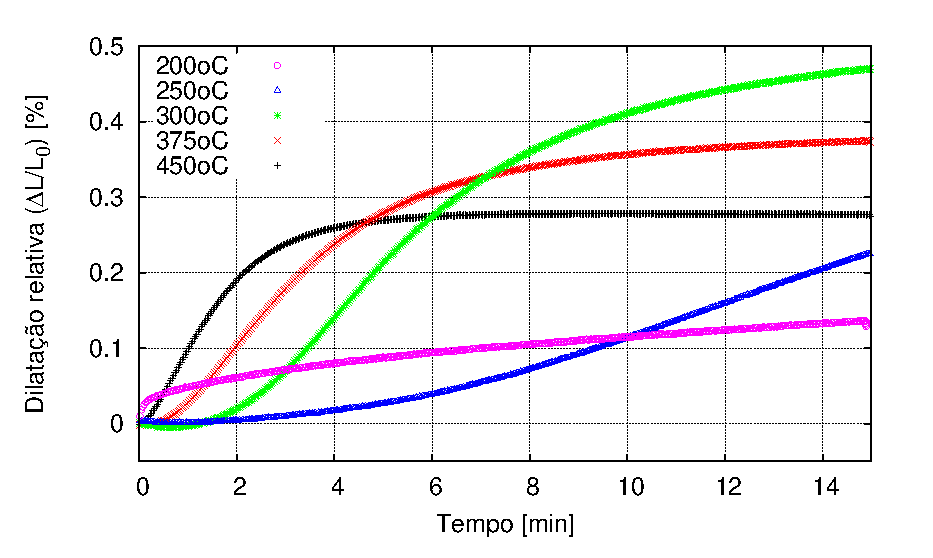
\includegraphics[width=.8\textwidth]{img/dilatometria/dlxt_austempera.eps}
	\end{figure}
\end{frame}

%%%Temperatura de têmpera

\begin{frame}{Resultados}{Influência da temperatura de têmpera}
	Efeito da temperatura de têmpera: 3 temperaturas de têmpera (140, 170 e 200) + amostra austemperada
	\begin{itemize}
		\item TP = 300 °C
	\end{itemize}
	
	\begin{figure}
		\centering
		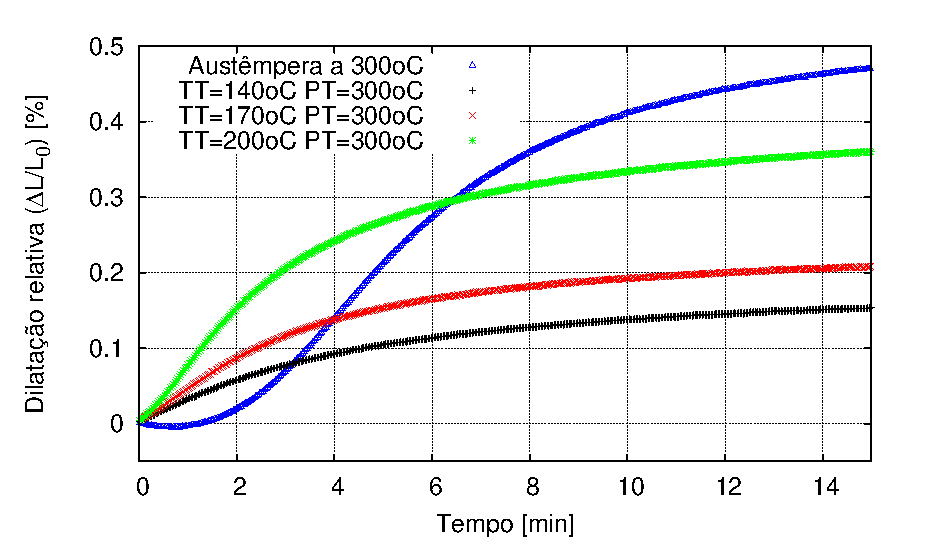
\includegraphics[width=.8\textwidth]{img/dilatometria/dlxt_PT300.eps}
	\end{figure}
\end{frame}

\begin{frame}{Resultados}{Influência da temperatura de têmpera}
	Amostras austemperadas apresentam tempo de incubação, enquanto amostras T\&P não. Possíveis hipóteses:
	\begin{itemize}
		\item Um tamanho de grão de $\gamma$ reduzido implica em menor temperabilidade
		\item A formação de $\alpha\text{'}$ gera tensões e defeitos cristalinos (discordâncias) em $\gamma$, facilitando a nucleação
		\item \textbf<2>{O processo de nucleação acontece durante o aquecimento desde TT até TP}
	\end{itemize}
\end{frame}

\begin{frame}{Resultados}{Influência da temperatura de têmpera}
	\begin{itemize}
		\item Aquecimento suficiente rápido pode evitar nucleação entre TT e TP
	\end{itemize}

	\begin{figure}
		\centering
		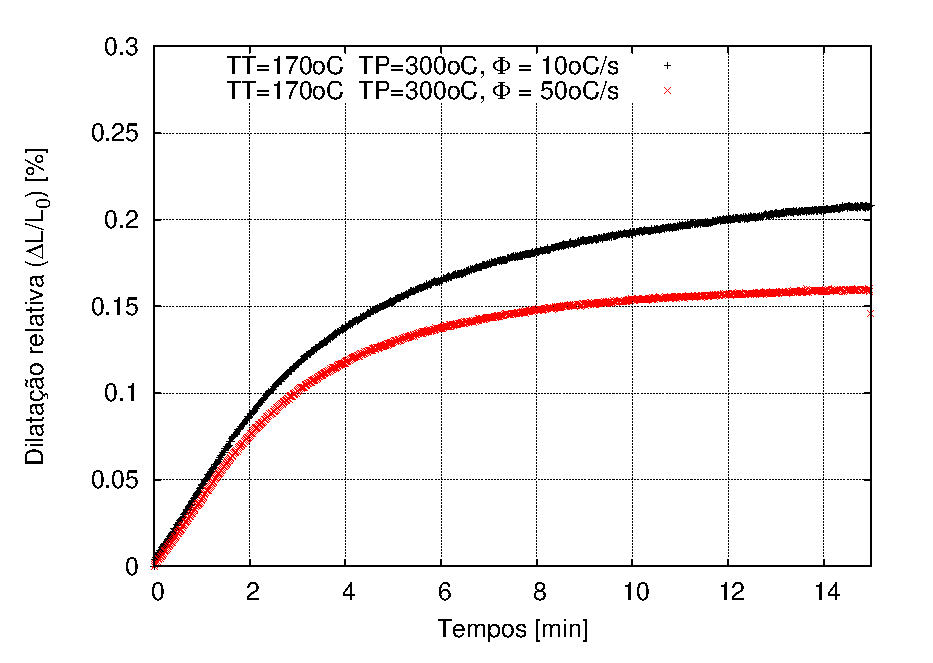
\includegraphics[width=.7\textwidth]{img/dilatometria/dlxt_heating.eps}
	\end{figure}

	\begin{itemize}
		\item Diferentes expansões, mas incubação não ocorre mesmo assim
	\end{itemize}
\end{frame}

\begin{frame}{Resultados}{Influência da temperatura de têmpera}
	\begin{itemize}
		\item \textbf<2>{Um tamanho de grão de $\gamma$ reduzido implica em menor temperabilidade}
		\item A formação de $\alpha\text{'}$ gera tensões e defeitos cristalinos (discordâncias) em $\gamma$, facilitando a nucleação
		\item \sout{O processo de nucleação acontece durante o aquecimento desde TT até TP}
	\end{itemize}
\end{frame}

\begin{frame}{Resultados}{Influência da temperatura de têmpera}
	\begin{itemize}
		\item A simples redução do tamanho de grão realmente aumenta a área da superfície
	\end{itemize}

	\begin{figure}
		\centering
		\includegraphics[width=.6\textwidth]{img/modelos/TG_aust.pdf}
	\end{figure}

	\begin{itemize}
		\item No T\&P é, na verdade, um pouco diferente: a nova fase não pode crescer para dentro de $\alpha\text{'}$!
		\item Ou seja, formação de $\alpha\text{'}$ realmente diminui a área interfacial?
	\end{itemize}

	\begin{figure}
		\centering
		\includegraphics[width=.6\textwidth]{img/modelos/TG_mart.pdf}
	\end{figure}
\end{frame}


\begin{frame}{Resultados}{Influência da temperatura de têmpera}
	\begin{figure}
		\centering
		\includegraphics[width=.6\textwidth]{img/modelos/TG_mart_2.pdf}
	\end{figure}

	Área superficial do grão original de $\gamma$
	\begin{equation*}
		S_{\gamma_0} = 4\cdot1 = \unit[4]{u.c.}
	\end{equation*}

	Área dos grãos de $\gamma$ não-transformados
	\begin{equation*}
		S_{\gamma_{nt}^1} = 2 \left[ 2 \left(\frac{1-a_1}{2}\right) + 2\cdot1 \right] = (6 - 2\cdot a_1)
	\end{equation*}

	\begin{equation*}
		S_{\gamma_{nt}^2} = 2 \left[ \left( \sqrt{2} - a_2 \right) + 2 \left( 1 - \frac{a_2}{\sqrt{2}} \right) \right] = 2\left(\sqrt{2} + 2\right)  - 2\left(\sqrt{2} + 1\right) a_2
	\end{equation*}
\end{frame}

\begin{frame}{Resultados}{Influência da temperatura de têmpera}
	\begin{figure}
		\centering
		\includegraphics[width=.8\textwidth]{img/modelos/Svsa.eps}
	\end{figure}

	\begin{itemize}
		\item Dependendo da geometria e da fração transformada, a formação de $\alpha\text{'}$ pode mesmo diminuir a área superficial de $\gamma$
		\item Formação de $\alpha\text{'}$ pode, portanto, \underline{aumentar} temperabilidade da austenita não-transformada
	\end{itemize}
\end{frame}

\begin{frame}{Resultados}{Influência da temperatura de têmpera}
	\begin{itemize}
		\item \sout{Um tamanho de grão de $\gamma$ reduzido implica em menor temperabilidade}. Depende!
		\item \textbf{A formação de $\alpha\text{'}$ gera tensões e defeitos cristalinos (discordâncias) em $\gamma$, facilitando a nucleação}
		\item \sout{O processo de nucleação acontece durante o aquecimento desde TT até TP}
	\end{itemize}
\end{frame}

\subsubsection{Análise não isotérmica}

\begin{frame}{Resultados}{Reações durante etapas não isotérmicas}
	\begin{itemize}
		\item<1> Partição por 2 h
			\begin{itemize}
				\item Decomposição de $\gamma$ começa antes de TP = 375, 450 °C ser atingida
			\end{itemize}
		\item<2> Partição por 15 min
			\begin{itemize}
				\item Formação de $\alpha\text{'}$ durante resfriamento final
			\end{itemize}
	\end{itemize}
	
	\begin{figure}
		\centering
		\includegraphics<1>[width=.78\textwidth]{/home/arthur/texto_tese/img/dilatometria/dlxT_qPTfc.pdf}
		\includegraphics<2>[width=.78\textwidth]{/home/arthur/texto_tese/img/dilatometria/dlxT_qPT15min-fc.pdf}
	\end{figure}
\end{frame}

%\begin{frame}[label=estimativaDil]{Resultados}{Resposta dilatométrica durante ciclo T\&P}
	%\begin{block}{Estimativa de $\Delta\%w_C^\gamma$ por dilatometria}
	%\begin{itemize}
		%\item Variação na temperatura Ms pode ser interpretada pelo enriquecimento em carbono da austenita
		%\item Ms da austenita antes da partição: 230 °C
		%\item Equação de Andrews: $Ms = 539 - 423\%w_C^\gamma - \dots$\\
			%logo: $\Delta\%w_C^\gamma = \frac{\Delta Ms}{423} = \frac{230 - Ms}{423}$
	%\end{itemize}
%
	%\begin{columns}
		%\begin{column}{0.5\textwidth}
		%\scalebox{0.85}{
			%\begin{tabular}{c c c c}
			%\hline
			%TT [°C] & TP [°C] & Ms [°C] & $\Delta\%w_C^\gamma$\\
			%\hline
			%140 & 200 & 119 & 0,26\\
			%170 & 200 & 148 & 0,19\\
			%200 & 200 & 168 & 0,15\\
			%\hline
			%140 & 250 & 35 & 0,46\\
			%170 & 250 & 77 & 0,36\\
			%200 & 250 & 109 & 0,29\\
			%\hline
			%140 & 300 & < 25 & > 0,48\\
			%170 & 300 & < 25 & > 0,48\\
			%200 & 300 & < 25 & > 0,48\\
			%\hline
			%\end{tabular}
		%}
		%\end{column}
%
		%\begin{column}{0.5\textwidth}
		%\scalebox{0.85}{
			%\begin{tabular}{c c c c}
			%\hline
			%TT [°C] & TP [°C] & Ms [°C] & $\Delta\%w_C^\gamma$\\
			%\hline
			%140 & 375 & < 25 & > 0,48\\
			%170 & 375 & < 25 & > 0,48\\
			%200 & 375 & < 25 & > 0,48\\
			%\hline
			%140 & 450 & < 25 & -\\
			%170 & 450 & < 25 & -\\
			%200 & 450 & < 25 & -\\
			%\hline
			%&&&\\
			%&&&\\
			%&&&\\
			%\end{tabular}
		%}
		%\end{column}
	%\end{columns}
	%\end{block}
	%\hyperlink{medidaDRX}{\beamerbutton{}}
%\end{frame}